\documentclass{article}
\usepackage{amsmath, amssymb}
\usepackage{listings}
\usepackage{enumerate}
\usepackage{bm}
\usepackage{fullpage}
\usepackage{empheq}
\usepackage{graphicx}
\usepackage{caption}
\usepackage{subcaption}
\usepackage{todonotes}

\title{CS 267 Parallel Computing Homework 2\\
\large{Part I (Serial \& OpenMP)}}
\author{Chiyu ``Max" Jiang, Eleanor Cawthon, Madeleine Traverse}
\usepackage[utf8]{inputenc}
\usepackage{color}

\definecolor{mygreen}{rgb}{0,0.6,0}
\definecolor{mygray}{rgb}{0.5,0.5,0.5}
\definecolor{mymauve}{rgb}{0.58,0,0.82}

\lstset{ %
  backgroundcolor=\color{white},   % choose the background color; you must add
                                   % \usepackage{color} or \usepackage{xcolor}
  basicstyle=\ttfamily,        % the size of the fonts that are used for the code
  breakatwhitespace=false,         % sets if automatic breaks should only happen
                                   % at whitespace
  breaklines=true,                 % sets automatic line breaking
  captionpos=b,                    % sets the caption-position to bottom
  commentstyle=\color{mygreen},    % comment style
  deletekeywords={...},            % if you want to delete keywords from the
                                   % given language
  escapeinside={\%*}{*)},          % if you want to add LaTeX within your code
  extendedchars=true,              % lets you use non-ASCII characters; for
                                   % 8-bits encodings only, does not work with
                                   % UTF-8
  frame=single,	                   % adds a frame around the code
  keepspaces=true,                 % keeps spaces in text, useful for keeping
                                   % indentation of code (possibly needs
                                   % columns=flexible)
  keywordstyle=\color{blue},       % keyword style
  language=Python,                 % the language of the code
  otherkeywords={*,...},           % if you want to add more keywords to the set
  numbers=left,                    % where to put the line-numbers; possible
                                   % values are (none, left, right)
  numbersep=5pt,                   % how far the line-numbers are from the code
  numberstyle=\tiny\color{mygray}, % the style that is used for the line-numbers
  rulecolor=\color{black},         % if not set, the frame-color may be changed
                                   % on line-breaks within not-black text (e.g.
                                   % comments (green here))
  showspaces=false,                % show spaces everywhere adding particular
                                   % underscores; it overrides 'showstringspaces'
  showstringspaces=false,          % underline spaces within strings only
  showtabs=false,                  % show tabs within strings adding particular
                                   % underscores
  stepnumber=2,                    % the step between two line-numbers. If it's
                                   % 1, each line will be numbered
  stringstyle=\color{mymauve},     % string literal style
  tabsize=2,	                   % sets default tabsize to 2 spaces
  title=\lstname                   % show the filename of files included with
                                   % \lstinputlisting; also try caption instead
                                   % of title
}
\newcommand{\defeq}{\overset{\text{def}}{=}}
\begin{document}
\maketitle
\section{Introduction}
The primary objective of this project is to implement an $\mathcal{O}(n)$
complexity algorithm to simulate particle dynamics solely dependent on
short-range forces, and extend the serial implementation to a shared-memory
and a distributed memory implementation. We begin in
Section~\ref{section:impl} by describing our changes to the provided
implementations, and analyzing their theoretical and experimental complexity. We
then examine analyze the performance of our code using VTune in
Section~\ref{section:vtune}, and discuss potential further improvements.  We
conclude with an evaluate the scalability of our two parallel approaches in
Section~\ref{section:scale}.
\section{Implementation Notes and
Complexity}\label{section:impl}
\todo[inline]{Eleanor will add MPI to this}
\subsection{Getting Serial to $\mathcal{O}(\log n)$}\label{subection:serial}
\subsubsection{Barnes-Hut Tree}
The first algorithm we implemented utilizes a data-structure which is
called a Barnes-Hut Tree \cite{barnes1986hierarchical}.
Barnes-Hut Tree algorithm is essentially an order $\mathcal{O}(n\log n)$
algorithm. However since this algorithm is more generally extensible to particle
simulations that take into consideration the long-range force interaction and
provides an efficient framework for simplifying it, it is still of interest to
implement and compare this data structure with the binning method. The
Barnes-Hut tree data structure is based on the quad tree data structure.
Initializing the data structure involves breaking the simulation domain
into finer and finer quadrants until each quadrant contains at most one
particle. Organized in this way, clusters of particles can be represented by the
center of mass of the cluster. Under certain threshold conditions, this can
be a good enough approximation.  Since the depth of a balanced quad tree is
$\mathcal{O}(\log n)$, the complexity of this algorithm is $\mathcal{O}(n\log
n)$. This is not ideal in terms of efficiency compared to the binning method,
but it is significantly more efficient that the naive implementation which is
order $\mathcal{O}(n^2)$.

\subsubsection{Binning Method}
We used a binning method to implement the Serial code. By dividing the space
of the simulation into bins, we were able to do far fewer computations as
compared with the original code. For each particle, the
\texttt{apply\_forces()} function was only applied to the particles in that
particle's bin and in the bins that neighbored it, so for a given particle, the
runtime would be $\mathcal{O}(9b n)$ instead of $\mathcal{O}(n^2)$. For our
code, the slope of the line of best fit in the \todo{Eleanor or Madeleine will
look up what the graph is that gets us this number to clarify this} fit is
1.031.

We accomplished the binning by creating a matrix of C++ vectors, with each
position in the matrix representing a single bin. We recreated this matrix at
the start of each time step to adjust for the movement of the particles (which
may have switched bins). An improvement for the serial code would be to edit the
existing matrix instead of creating a new one, but since creating the matrix is
only an $\mathcal{O}(n)$ operation, we did not think the improvement would be
appreciable.

To find the optimal number of bins for the simulation, we set the minimum size
of the bin to the cutoff/100.  We then used a search to find the optimal bin
size. As shown in Figure~\ref{fig:bin_time}, we found 16 bins to be optimal for
reducing simulation time.

\begin{figure}[ht]
\centering
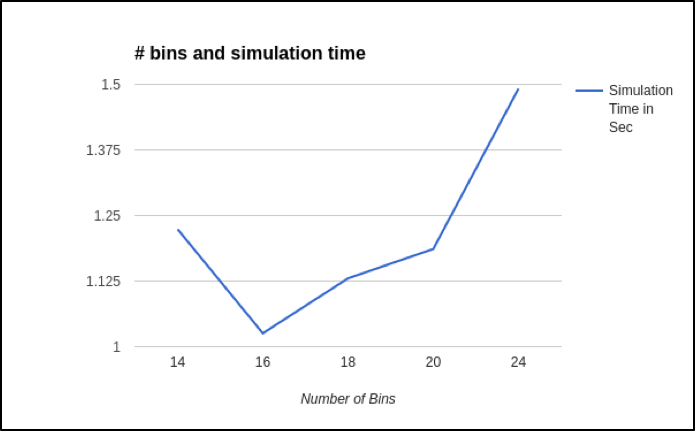
\includegraphics[width=0.7\textwidth]{Picture1.png}
\caption{Plot of number of bins vs. simulation time in the serial simulation.
  This plot indicates that optimal performance is achieved when the number of
  bins is set to 16.}
\label{fig:bin_time}
\end{figure}
\subsection{Shared Memory Implementation with OpenMP}
\label{subsection:openmp}
\subsubsection{Binning Method}
To create the OpenMP code, the serial code with binning was reorganized to allow
for OpenMP Pragmas. The comparing of the particles in the bin matrix was
parallelized by collapsing the matrix for loops into one long process that could
be divided between threads. The scheduler was set to dynamic, however no
statistically significant difference was observed between static and dynamic
allocation. We also attempted to parallelize the creation of the bin matrix at
the beginning of the timestep, but constant segfaults suggested that the code
was not compatible with the pragmas used as the threads were attempting to
create infinite bins.
\subsubsection{Barnes-Hut Tree}
In our first serial implementation of the Barnes-Hut Tree approach, we
re-created the entire particle tree every time the simulation moved to a new
step. Although this did not affect the Big-O runtime, this involved double the
amount of work per step, which is significant even though it is a constant
factor. It also made the code difficult to parallelize because the initial
construction of the tree requires synchronization, introducing a serialized
bottleneck. For these reasons, we decided it was important to enable our
implementation to make updates to the already-constructed tree, allowing
sub-trees to be updated in parallel. Unfortunately, implementing this
functionality proved substantially more difficult than expected, and we
ultimately abandoned this variant due to time constraints. As such, we did not
parallelize the Barnes-Hut variant.

\subsection{Complexity test}
\todo[inline]{Eleanor will add MPI to this}
Complexity test for the serial codes is acquired from the autograder. For better
visualization purposes, the results for simulation is plotted on a log-log
scale. Refer to Figures \ref{fig:loglogbin} and \ref{fig:loglogBH}.

It can be observed that with binning method, the overall average slope for
log-log plot is lower (1.1409), however the it shows an increasing trend in log
time for greater $n$. Barnes-Hut tree based algorithms shows more consistent
polynomial order performance regardless of $n$.

\begin{figure}[h!]
\centering
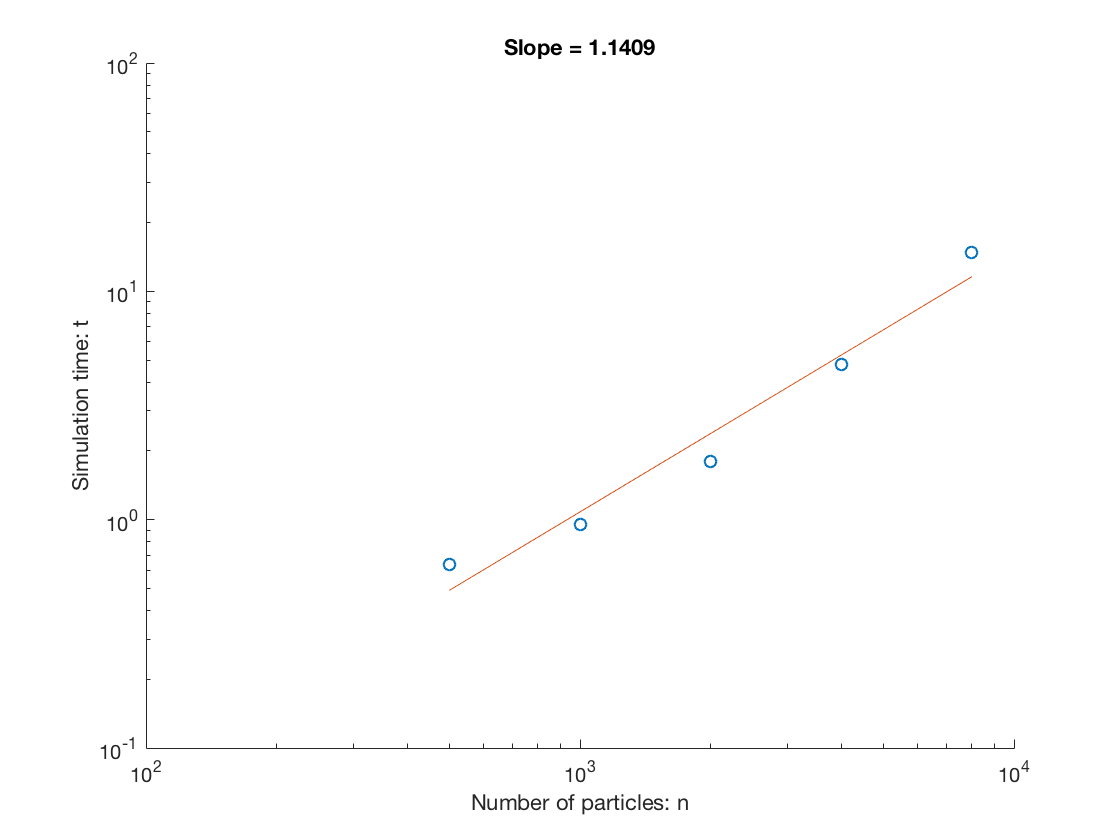
\includegraphics[width=0.7\textwidth]{Picture4.png}
\caption{log-log plot of number of particles versus simulation time for
performance analysis on binning method code.}\label{fig:loglogbin}
\end{figure}
\begin{figure}[h!]
\centering
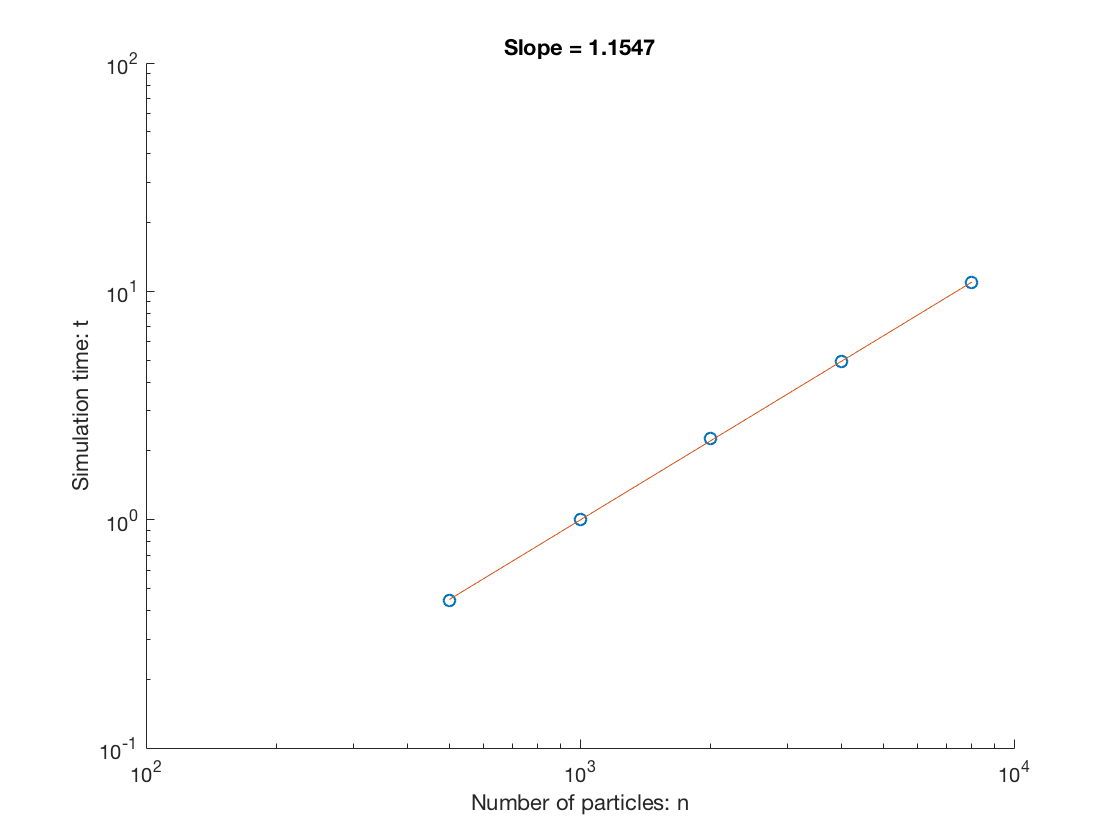
\includegraphics[width=0.7\textwidth]{Picture5.png}
\caption{log-log plot of number of particles versus simulation time for
performance analysis on Barnes-Hut method code.}\label{fig:loglogBH}
\end{figure}

\section{Performance Analysis}\label{section:vtune}
\todo[inline]{Madeleine will do this}
\section{Results At Scale}\label{section:scale}
\todo[inline]{Eleanor will finish this}
\begin{figure}[ht!]
\centering
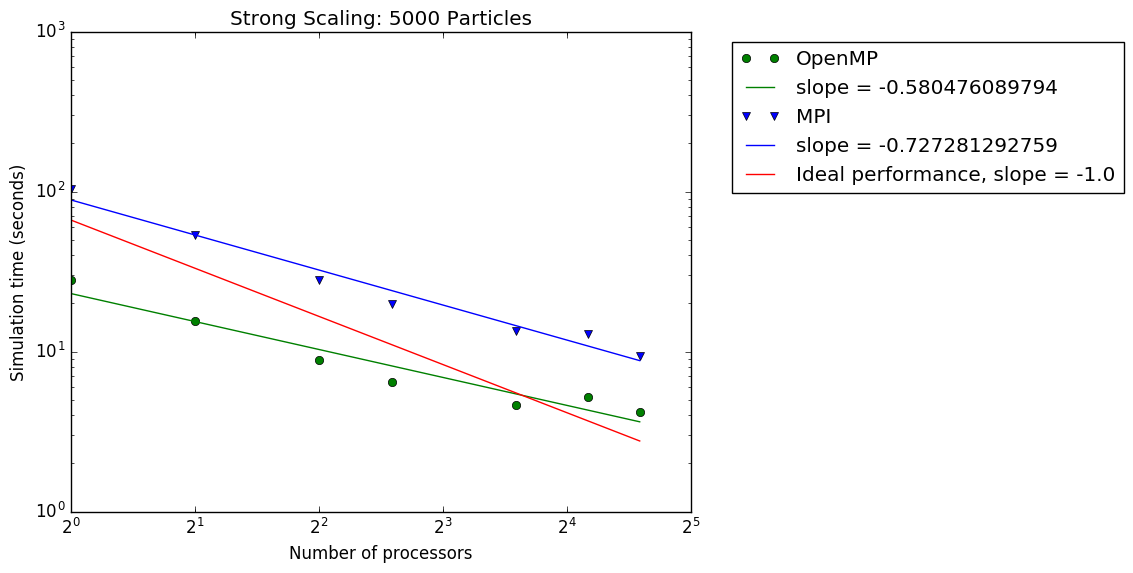
\includegraphics[width=0.7\textwidth]{strong.png}
\caption{Strong scaling results, OpenMP vs. MPI}\label{fig:strong}
\end{figure}
\begin{figure}[ht!]
\centering
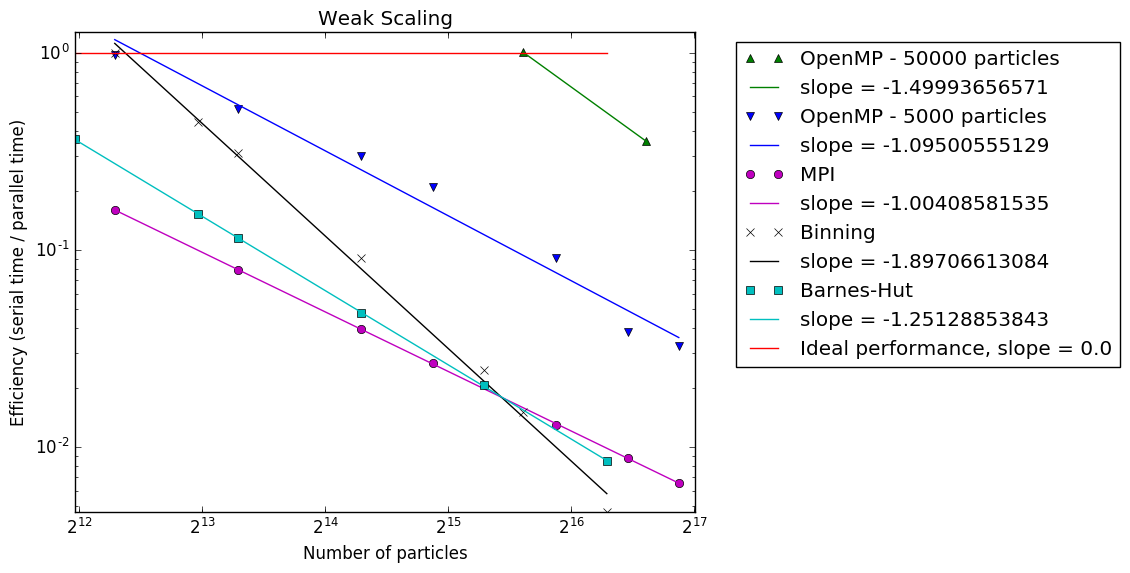
\includegraphics[width=0.7\textwidth]{weak.png}
\caption{Weak scaling results, OpenMP vs. MPI}\label{fig:weak}
\end{figure}
\subsection{Comparison between binning serial vs. OpenMP implementation}
Serial outperforms OpenMP in numbers of particles less than 2000. This makes
sense because the overhead needed for thread creation in OpenMP cannot be
ameliorated by the overall decrease in simulation time. However, once the number
of particles is more than 2000, OpenMP does vastly better. Serial struggles with
more particles in an accelerated rate, while OpenMP threads manage the increase
in particles with a linear increase.
\begin{figure}[h]
\centering
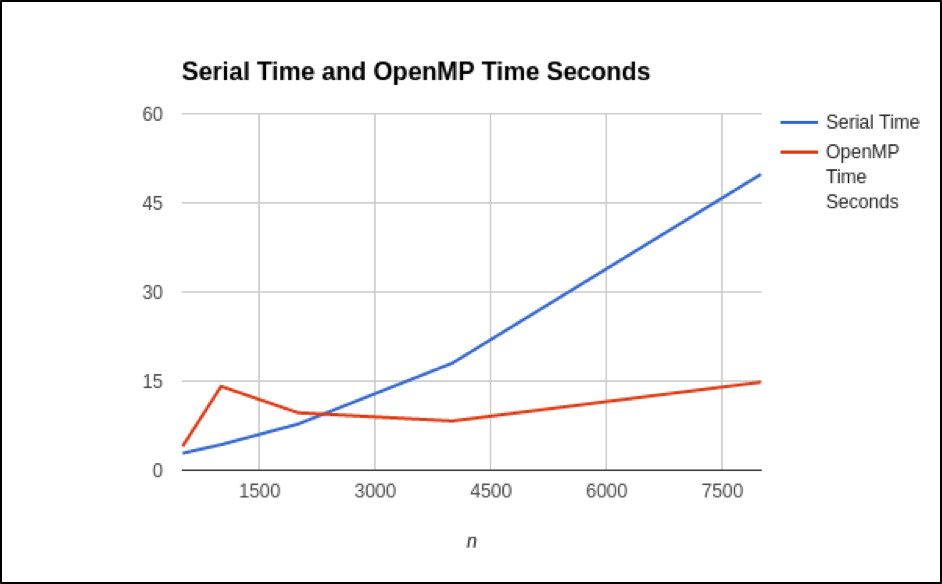
\includegraphics[width=0.7\textwidth]{Picture3.png}
\caption{Comparison between serial time and OpenMP implementations. $x$ axis
shows particle density and $y$ axis shows running time.}
\end{figure}
\clearpage
\bibliography{main.bib}
\bibliographystyle{unsrt}

\end{document}

